



%\definecolor{blueaccent}{RGB}{0,150,214}
%\definecolor{greenaccent}{RGB}{0,139,43}
%\definecolor{purpleaccent}{RGB}{130,41,128}
%\definecolor{orangeaccent}{RGB}{240,83,50}
%
%\addplot+[greenaccent,mark=*,mark options={fill=greenaccent}] table{results/NewExpt1/Expt3/comp_subsampled_CustomMOSS0RR1.txt};
%		\addplot+[purpleaccent,mark=*,mark options={fill=purpleaccent}] table{results/NewExpt1/Expt3/comp_subsampled_CustomOCUCB0RR1.txt};
%		\addplot+[orangeaccent,mark=*,mark options={fill=orangeaccent}] table{results/NewExpt1/Expt3/comp_subsampled_CustomEXP30RR1.txt};

%\begin{figure}[!th]
%\centering
%\begin{tabular}{c}
%\setlength{\tabcolsep}{0.1pt}
%\subfigure[0.25\textwidth][Expt-$1$: $1024$ Users, $128$ arms, Round-Robin, Noisy Setting, Rank $2$, equal sized clusters]
%    %with $r_{i_{{i}\neq {*}}}=0.07$ and $r^{*}=0.1$
%    {
%    		\pgfplotsset{
%		tick label style={font=\Large},
%		label style={font=\Large},
%		legend style={font=\Large},
%		ylabel style={yshift=5pt},
%		%legend style={legendshift=32pt},
%		}
%        \begin{tikzpicture}[scale=0.4]
%      	\begin{axis}[
%		xlabel={timestep},
%		ylabel={Cumulative Regret},
%		grid=major,
%        %clip mode=individual,grid,grid style={gray!30},
%        clip=true,
%        %clip mode=individual,grid,grid style={gray!30},
%  		legend style={at={(0.5,1.4)},anchor=north, legend columns=3} ]
%      	% UCB
%		
%		\addplot table{results/NewExpt2/Expt1/comp_subsampled_CustomTS0RR1.txt};
%		\addplot table{results/NewExpt2/Expt1/comp_subsampled_NewMetaEXP0RR1.txt};
%		\legend{TS, LRBandit} 
%      	\end{axis}
%      	\end{tikzpicture}
%  		\label{fig:0}
%    }
% \end{tabular}
%    \caption{A comparison of the cumulative regret by MRLG and MRLUCB. }
%    \label{fig:karmed}
%    \vspace*{-1em}
%\end{figure}

\begin{figure}[!th]
\centering
\begin{tabular}{cc}
\setlength{\tabcolsep}{0.1pt}
\subfigure[0.25\textwidth][Expt-$1$: $2048$ Users, $64$ Bernoulli-distributed arms, Round-Robin, Noisy Setting, Rank $2$, equal sized clusters]
    %with $r_{i_{{i}\neq {*}}}=0.07$ and $r^{*}=0.1$
    {
    		\pgfplotsset{
		tick label style={font=\Large},
		label style={font=\Large},
		legend style={font=\Large},
		ylabel style={yshift=5pt},
		%legend style={legendshift=32pt},
		}
        \begin{tikzpicture}[scale=0.4]
      	\begin{axis}[
		xlabel={timestep},
		ylabel={Cumulative Regret},
		grid=major,
        %clip mode=individual,grid,grid style={gray!30},
        clip=true,
        %clip mode=individual,grid,grid style={gray!30},
        cycle list name=exotic,
  		legend style={at={(0.5,1.4)},anchor=north, legend columns=3} ]
      	% UCB
		\addplot table{results/NewExpt1/Expt2/comp_subsampled_CustomTS0RR1.txt};
		\addplot table{results/NewExpt1/Expt2/comp_subsampled_MetaEXP0RR1.txt};
		\addplot table{results/NewExpt1/Expt2/comp_subsampled_MetaEXP0RR2.txt};
		\addplot table{results/NewExpt1/Expt2/comp_subsampled_CustomNMFG0RR1.txt};
		\addplot table{results/NewExpt1/Expt2/comp_subsampled_CustomNMF0RR1.txt};
		\addplot table{results/NewExpt1/Expt2/comp_subsampled_CustomOCUCB0RR1.txt};
		\legend{TS, LRUCB, LRG, NMFG, NMFUCB, OCUCB} 
      	\end{axis}
      	\end{tikzpicture}
  		\label{fig:1}
    }
    &
    \subfigure[0.25\textwidth][Expt-$2$: $2048$ Users, $64$ Bernoulli-distributed arms, Round-Robin, Noisy Setting, Rank $2$, un-equal sized clusters, 70:30 split]
    %with $r_{i_{{i}\neq {*}}}=0.07$ and $r^{*}=0.1$
    {
    		\pgfplotsset{
		tick label style={font=\Large},
		label style={font=\Large},
		legend style={font=\Large},
		ylabel style={yshift=5pt},
		%legend style={legendshift=32pt},
		}
        \begin{tikzpicture}[scale=0.4]
      	\begin{axis}[
		xlabel={timestep},
		ylabel={Cumulative Regret},
		grid=major,
        %clip mode=individual,grid,grid style={gray!30},
        clip=true,
        %clip mode=individual,grid,grid style={gray!30},
        cycle list name=exotic,
  		legend style={at={(0.5,1.4)},anchor=north, legend columns=3} ]
      	% UCB
		\addplot table{results/NewExpt1/Expt3/comp_subsampled_CustomTS0RR1.txt};
		\addplot table{results/NewExpt1/Expt3/comp_subsampled_MetaEXP0RR1.txt};
		\addplot table{results/NewExpt1/Expt3/comp_subsampled_MetaEXP0RR2.txt};
		\addplot table{results/NewExpt1/Expt3/comp_subsampled_CustomNMFG0RR1.txt};
		\addplot table{results/NewExpt1/Expt3/comp_subsampled_CustomNMF0RR1.txt};
		\addplot table{results/NewExpt1/Expt3/comp_subsampled_CustomOCUCB0RR1.txt};
		\legend{TS, LRUCB, LRG, NMFG, NMFUCB, OCUCB} 
      	\end{axis}
      	\end{tikzpicture}
  		\label{fig:2}
    }
    \\
    \subfigure[0.25\textwidth][Expt-$3$: $4096$ Users, $128$ Bernoulli-distributed arms, Round-Robin, Noisy Setting, Rank $2$, equal sized clusters]
    %with $r_{i_{{i}\neq {*}}}=0.07$ and $r^{*}=0.1$
    {
    		\pgfplotsset{
		tick label style={font=\Large},
		label style={font=\Large},
		legend style={font=\Large},
		ylabel style={yshift=5pt},
		%legend style={legendshift=32pt},
		}
        \begin{tikzpicture}[scale=0.4]
      	\begin{axis}[
		xlabel={timestep},
		ylabel={Cumulative Regret},
		grid=major,
        %clip mode=individual,grid,grid style={gray!30},
        clip=true,
        %clip mode=individual,grid,grid style={gray!30},
        cycle list name=exotic,
  		legend style={at={(0.5,1.4)},anchor=north, legend columns=3} ]
      	% UCB
		\addplot table{results/NewExpt1/Expt4/comp_subsampled_CustomTS0RR1.txt};
		\addplot table{results/NewExpt1/Expt4/comp_subsampled_MetaEXP0RR1.txt};
		\addplot table{results/NewExpt1/Expt4/comp_subsampled_MetaEXP0RR2.txt};
		\addplot table{results/NewExpt1/Expt4/comp_subsampled_CustomNMFG0RR1.txt};
		\addplot table{results/NewExpt1/Expt4/comp_subsampled_CustomNMF0RR1.txt};
		\addplot table{results/NewExpt1/Expt4/comp_subsampled_CustomOCUCB0RR1.txt};
		\legend{TS, LRUCB, LRG, NMFG, NMFUCB, OCUCB} 
      	\end{axis}
      	\end{tikzpicture}
  		\label{fig:3}
    }
    &
    \subfigure[0.25\textwidth][Expt-$4$: $4096$ Users, $128$ Bernoulli-distributed arms, Round-Robin, Noisy Setting, Rank $2$, un-equal sized clusters, 80:20 split]
    %with $r_{i_{{i}\neq {*}}}=0.07$ and $r^{*}=0.1$
    {
    		\pgfplotsset{
		tick label style={font=\Large},
		label style={font=\Large},
		legend style={font=\Large},
		ylabel style={yshift=5pt},
		%legend style={legendshift=32pt},
		}
        \begin{tikzpicture}[scale=0.4]
      	\begin{axis}[
		xlabel={timestep},
		ylabel={Cumulative Regret},
		grid=major,
        %clip mode=individual,grid,grid style={gray!30},
        clip=true,
        %clip mode=individual,grid,grid style={gray!30},
        cycle list name=exotic,
  		legend style={at={(0.5,1.4)},anchor=north, legend columns=3} ]
      	% UCB
		\addplot table{results/NewExpt1/Expt5/comp_subsampled_CustomTS0RR1.txt};
		\addplot table{results/NewExpt1/Expt5/comp_subsampled_MetaEXP0RR1.txt};
		\addplot table{results/NewExpt1/Expt5/comp_subsampled_MetaEXP0RR2.txt};
		\addplot table{results/NewExpt1/Expt5/comp_subsampled_CustomNMFG0RR1.txt};
		\addplot table{results/NewExpt1/Expt5/comp_subsampled_CustomNMF0RR1.txt};
		\addplot table{results/NewExpt1/Expt5/comp_subsampled_CustomOCUCB0RR1.txt};
		\legend{TS, LRUCB, LRG, NMFG, NMFUCB, OCUCB} 
      	\end{axis}
      	\end{tikzpicture}
  		\label{fig:4}
    }
    \end{tabular}
    \caption{A comparison of the cumulative regret incurred by the various bandit algorithms. }
    \label{fig:karmed1}
    \vspace*{-1em}
\end{figure}





%[[1104, 99], [896, 93],[0,0][0,0]}

\begin{figure}[!th]
\centering
\begin{tabular}{c}
\setlength{\tabcolsep}{0.1pt}
\subfigure[0.25\textwidth][Expt-$1$: $2000$ Users, $100$ arms, Round-Robin, Noisy Setting, Rank $2$, Jester Dataset]
    %with $r_{i_{{i}\neq {*}}}=0.07$ and $r^{*}=0.1$
    {
    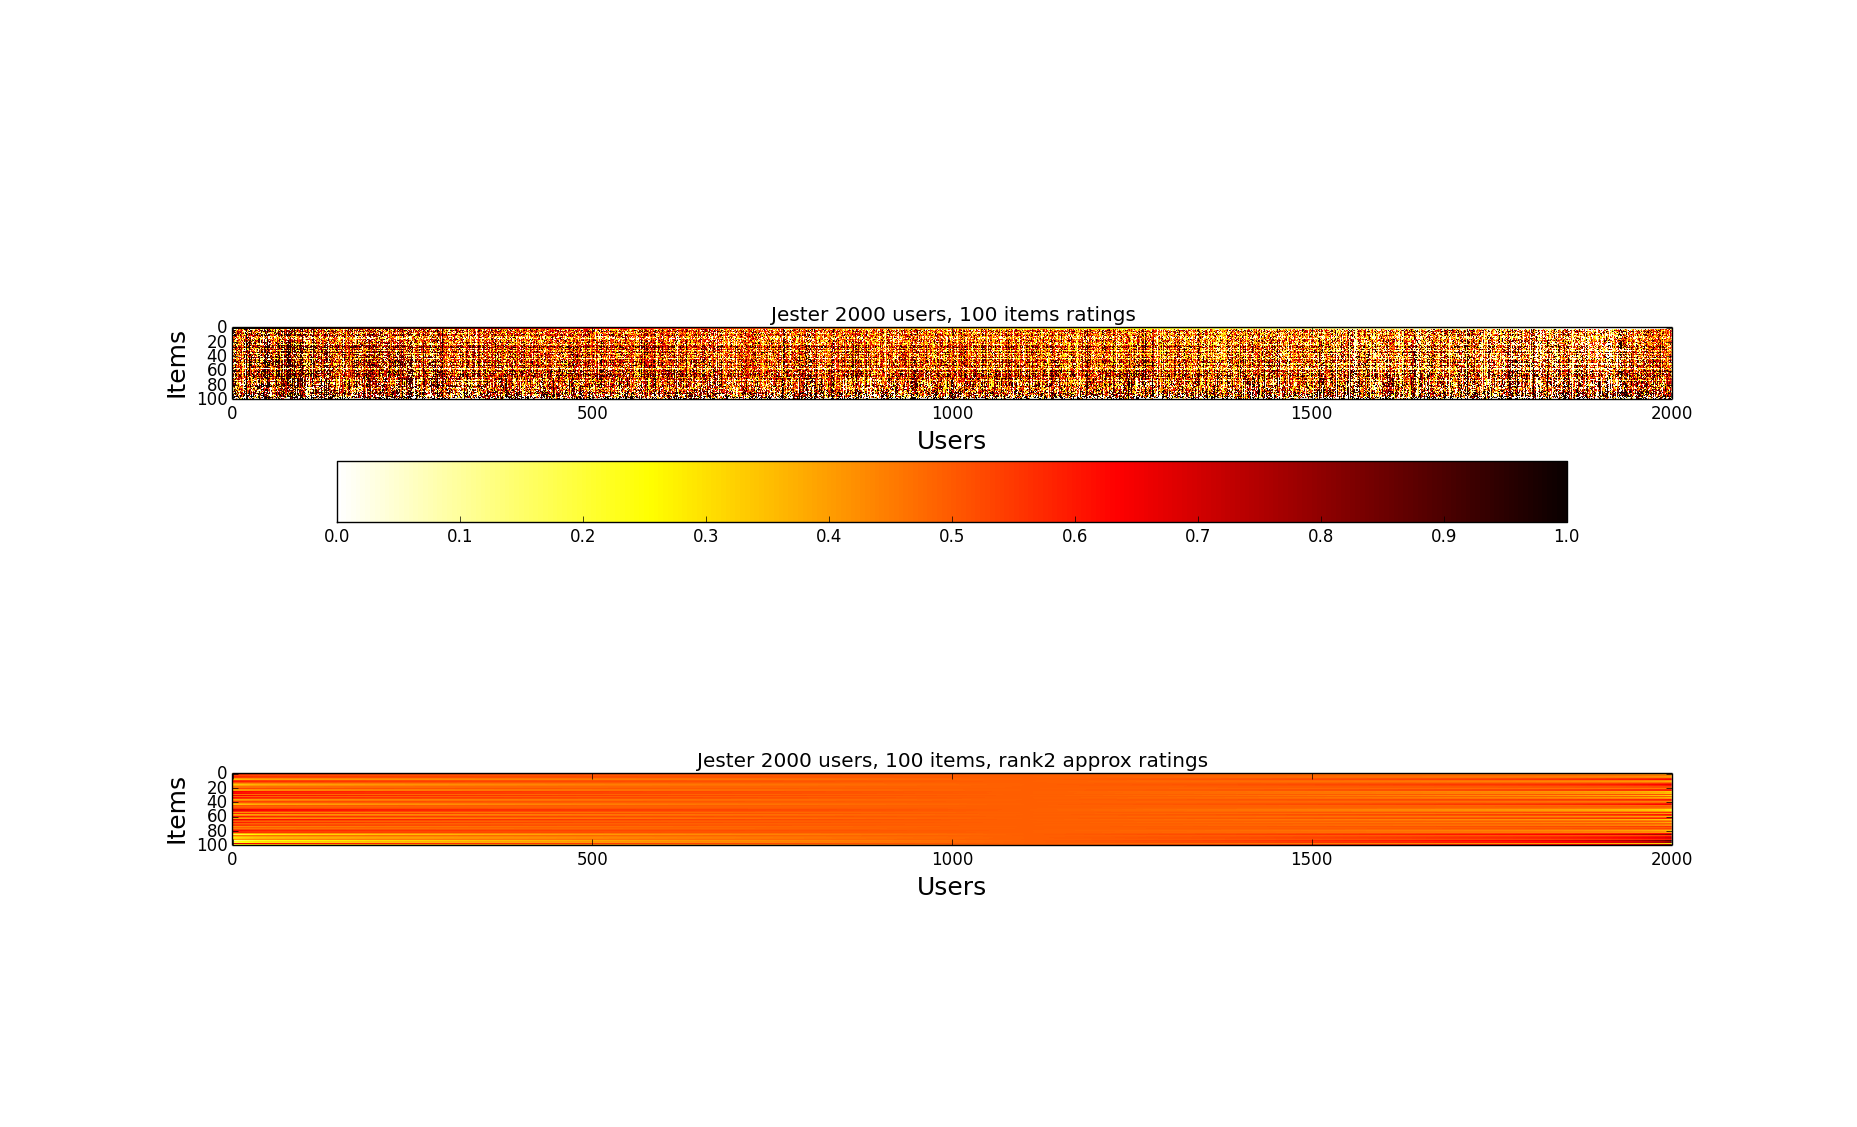
\includegraphics[scale=0.2]{img/jester_rank2.png}
    	\label{fig:5}
    }
    \\
\subfigure[0.25\textwidth][Expt-$1$: $2000$ Users, $100$ arms, Round-Robin, Noisy Setting, Rank $2$, Jester Dataset]
    %with $r_{i_{{i}\neq {*}}}=0.07$ and $r^{*}=0.1$
    {
    		\pgfplotsset{
		tick label style={font=\Large},
		label style={font=\Large},
		legend style={font=\Large},
		ylabel style={yshift=5pt},
		%legend style={legendshift=32pt},
		}
        \begin{tikzpicture}[scale=0.4]
      	\begin{axis}[
		xlabel={timestep},
		ylabel={Cumulative Regret},
		grid=major,
        %clip mode=individual,grid,grid style={gray!30},
        clip=true,
        cycle list name=exotic,
        %clip mode=individual,grid,grid style={gray!30},
  		legend style={at={(0.5,1.4)},anchor=north, legend columns=3} ]
      	% UCB
		
		\addplot table{results/NewExpt3/Expt1/comp_subsampled_CustomTS0RR1.txt};
		\addplot table{results/NewExpt3/Expt1/comp_subsampled_MetaEXP0RR1.txt};
		\addplot table{results/NewExpt3/Expt1/comp_subsampled_MetaEXP0RR1G.txt};
		\addplot table{results/NewExpt3/Expt1/comp_subsampled_CustomNMFG0RR2.txt};
		\addplot table{results/NewExpt3/Expt1/comp_subsampled_CustomNMF0RR1.txt};
		\addplot table{results/NewExpt3/Expt1/comp_subsampled_CustomOCUCB0RR1.txt};
		\legend{TS, LRUCB, LRG, NMFG, NMFUCB, OCUCB} 
      	\end{axis}
      	\end{tikzpicture}
  		\label{fig:6}
    }
 \end{tabular}
    \caption{A comparison of the cumulative regret in Jester Dataset }
    \label{fig:karmed}
    \vspace*{-1em}
\end{figure}